\chapter{Network Models}\label{network_models}


%% Collectors Profiling and activities history
%%%% Profiling collectors in terms of their activities and interests can be a way of further detecting anomalies (activity monitoring, Fawcett and Provost 1999).


\begin{figure}[h!]
  	\centering
    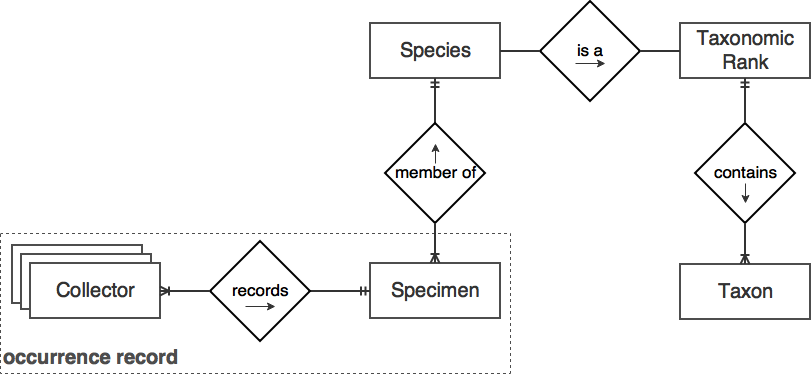
\includegraphics[width=0.8\linewidth]{figures/er_occurrence.png}
    \caption{Entity-relationship diagram for occurrences.}
    \label{fig:er_occurrences}
\end{figure}

This chapter contains the core models I've developed during this study.
% What am I modeling with these models?

Here a distinction must be stated for the terms "species" and "specimen" I'll constantly refer to along this text. The former refers to a taxonomic rank, a group of individuals forming a biological classification unit as determined by a professional taxonomist. The latter refers to an individual, which can be identified as being a representative of one species. These relationships are illustrated in Figure \ref{fig:er_occurrences}.

After properly deposited in a biological collection, each record receives a taxonomic identification that assigns the individual to a taxonomic group (a taxon), in a best-effort manner.

\section{Complex Networks: A theoretical background}
\subsection{The rise of the study of complex networks}
%% The rise of the field of complex networks
%% A historical background
%% Applications (biology and other fields)
%% What are complex networks?
%%%% Random networks, small-world and scale-free topologies

\subsection{Mathematical Representations}
% Networks are mathematically represented as graphs
%% Nodes and Edges
%%% Edges are established between a pair of nodes , recurrent edges
%%% Nodes and edges can have attributes (each attribute holding values)
%%% Neighborhood, neighbors
%%% Cliques
%%% Paths 

%% Graph density
%%% Fully connected: n*(n-1)/2


%% Matrix Representation
%%% Adjacency matrix, sparsity

%% Degree
%%%% Degree distribution
%%%% Power laws
%%%%% Many real-world networks are approximately scale-free (give examples)
%%%% Machanism: Preferential attachment, rich gets richer: Higher degree nodes (richer), lower degree nodes (poorer)

\subsection{Bipartite Graphs}
%% Bipartite graphs
%%%% The bipartite constraint: formalization: Nodes sets are DISJOINT (no intersection) ; and INDEPENDENT (no adjacent nodes within any set); 
%%%% Biadjacency matrix
%%%% Bipartite projection
%%%%%% bipartite projections edges set is usually very dense -> The importance of adding weights to edges in bipartite projections
%%%%%% weaker connections are then filtered out

  \begin{figure}[h!]
  	\centering
    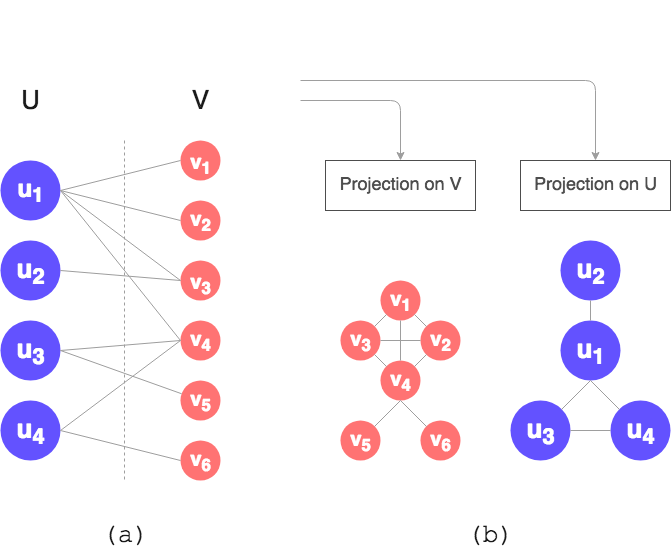
\includegraphics[width=0.5\linewidth]{figures/bipartite_general.png}
    \caption{(a) General aspect of a bipartite graph. All nodes in the graph belong to exactly one of $U$ and $V$ nodes sets. In addition edges are only established between nodes from distinct sets. (b) Bipartite projections. Projections onto each node set are constructed by linking together nodes that are at a length-2 distance in the bipartite graph, while omitting nodes from the other set.}
    \label{fig:bipartite_general}
  \end{figure}


\section{Species-collectors Networks}

%% Goals and Questions to investigate
%% TODO: SCNs do not allow 0-degree nodes


\subsection{General description}

Species-collectors networks (SCN) describe relationships of the type ``\textbf{collector} samples \textbf{species}'' or, conversely, ``\textbf{species} is sampled by \textbf{collector}''. 
As such relationships can only possibly exist between collectors and species we explicitly represent collectors and species as entities belonging to distinct entity classes. Additionally, we add a constraint only allowing links to be established between collectors and species.
As all relationships in the network necessarily involve one entity belonging to each class it is best described by a bipartite graph model
$$ SCN = (S_{sp},S_{col},E) \mbox{ ,}$$
where $S_{col}$ is the nodes set representing the collectors group; $S_{sp}$ is the nodes set representing the species group; and $E$ is the set of undirected edges between members of $S_{col}$ and $S_{sp}$.

% https://www.latex-tutorial.com/tutorials/figures/
  \begin{figure}[h!]
  	\centering
    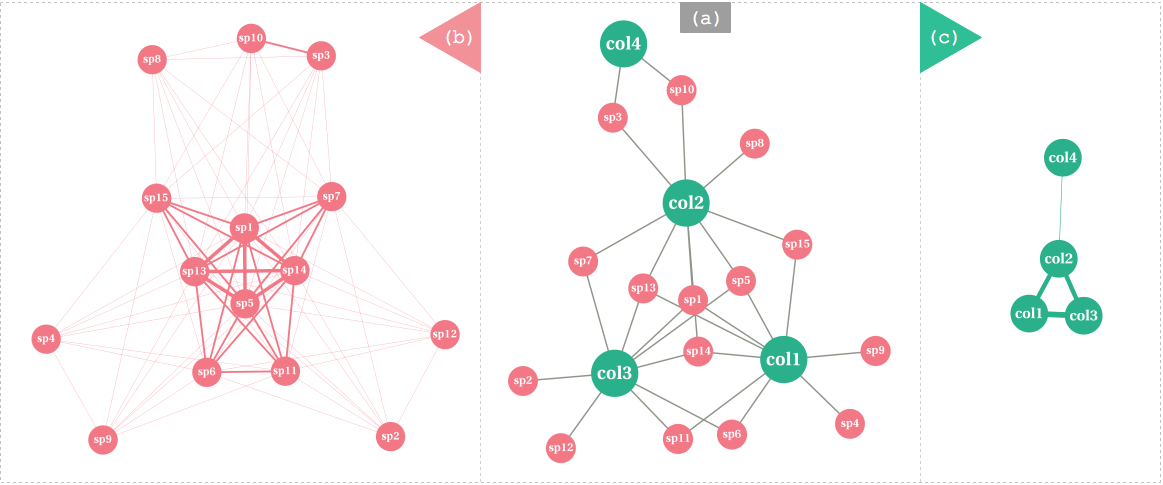
\includegraphics[width=\linewidth]{figures/scn_generalaspect.png}
    \caption{(a) General aspect of a species-collectors network model (SCN), where collectors are linked to the species they've recorded. The total number of records of a given species by some collector is reflected in the strength of their link. Here for simplicity all collectors have recorded each species once. (b) SCN projection onto the species set. Species are linked together if they've been collected by common collectors. Link strength is proportional to the number of collectors two species share. (c) SCN projection onto the collectors set. Collectors are linked together if they've recorded species in common. Link strength is proportional to the number of species two collectors share. Link strength in each network is graphically represented by edges thickness.}
    \label{fig:scn_general}
  \end{figure}

Note that in this model entities from the collectors class represent actual individuals (people), whereas each entity from the species class refer instead to a species, which by definition comprises a group of individuals. 
Therefore new links between nodes are formed whenever a collector records an individual belonging to a new species. 
For new occurrences of already existent species-collector pairs no new edges are added. Instead, the weights of those edges are increased, such that the final weight of each edge corresponds to the total number of times a given collector has recorded a given species.

Nodes and edges in a SCN model can also be represented as a rectangular \textit{biadjacency matrix} $A$ with dimensions $|S_{sp}|\times|S_{col}|$, wherein each element represents the number of records of a particular species by some collector.

Below I introduce some basic definitions in the scope of SCN models.

%% SCN definitions
\paragraph{Species bag.} 
The entire set and counts of species a collector has recorded in a dataset, which is equivalent to the set formed by the node's direct neighbors, composes his/her \textit{species bag}.
Species bag is an attribute which is exclusively derived for collectors nodes, formally defined as a vector
$$
\sigma^{(\mu)} =  \begin{bmatrix}
\sigma_1^{(\mu)}, \sigma_2^{(\mu)}, \cdots, \sigma_n^{(\mu)}
\end{bmatrix}  \quad : \quad 
n = |S_{sp}|
$$
where $n$ is the length of the species set and each $\sigma_i^{(\mu)}$ is the total number of records of species $i$ by collector $\mu$. 
The species bag can be directly obtained as a row-vector from the SCN biadjacency matrix.
The sum of all elements in a collector's species bag is given by the species bag's \textit{l1 norm} $|| \sigma^{(\mu)} ||_1$, and corresponds to the node's \textit{weighted degree} $k_w$.\todo{review weighted degree definition}
 
\paragraph{Interest.} 
The entire set and counts of collectors that have recorded a particular species in a dataset is defined as its \textit{interest} vector. This concept can be thought as the inverse of a species bag, being equivalent to the nodes set formed by a species' direct neighbors. The interest vector is an attribute derived exclusively for species nodes, and is formally defined as
$$ 
\iota^{(\psi)} =  \begin{bmatrix}
\iota^{(\psi)}_1, \iota_2^{(\psi)}, \cdots, \iota_n^{(\psi)}
\end{bmatrix}  \quad : \quad 
n = |S_{col}|
$$
where $n$ is the length of the collectors set and each $\iota_i^{(\psi)}$ is the total number of records of species $\psi$ which was done by collector $i$. 
A particular species' interest can also be derived as a column-vector from the biadjacency matrix. 
The weighted degree $k_w$ \todo{review weighted degree definition}of a species node can also be derived by computing the \textit{l1-norm} of its interest vector, such that $k_w^{(\psi)} \equiv || \iota^{(\psi)} ||_1 $.

\paragraph{Taxonomic aggregation and resolution.}
In some contexts it might be desired to simplify SCNs by grouping species nodes into higher taxonomic ranks (or levels), such as \textit{genus} or \textit{family}. This process is defined as \textit{taxonomic aggregation}, and is performed by 
($i$) obtaining a grouping of species using some taxonomic rank; 
($ii$) obtaining interest vectors for each species; 
($iii$) summing up interest vectors for all species in each group;
($iv$) building a new SCN model, aggregated on rank T. 
The SCN's \textit{taxonomic resolution} is the taxonomic rank at which species are aggregated in the model. For the sake of model interpretability, all nodes in $S_{sp}$ must necessarily be represented as taxons belonging to the same rank as the SCN's taxonomic resolution.

For a more formal description let $G_T = \{ g_1, g_2, \cdots, g_n \}$ be a taxonomic grouping at rank $T$ containing a set of taxons $g_i$, each of them mapping to a set of species nodes $S_{sp}^{(i)} \subset S_{sp}$. Then for each node $g_i \in G_T$ we obtain their interest vectors by computing $ \iota^{(g_i)} := \sum_{j=1}^{m} \iota^{(v_j)} : v_j \in S_{sp}^{(i)}, m = |g_i|$. By stacking all interests vector as row-vectors we obtain a biadjacency matrix, which is then used to build a rank-T aggregated SCN model $SCN_T = (G_T,S_{col},E)$.
% The PICI model (Lambiotte2005)
%% Collective effects acting on individuals with similar interests
%% Individual mechanisms, pushing collectors towards their particular interests, establishing their collecting niche

% Temporal edges

% Model metrics
\subsection{Metrics and attributes}
In this section I describe metrics and attributes of nodes and edges in the model.

\paragraph*{Specificity.} 
% This metric doesn't work well for very low degrees with very high weighted degrees (for example in aggregations into family level)
How many of a collector's new records refer to species he/she had never recorded before?
Is a particular species mostly collected by the same collector or are there many other collectors that are also interested in it?
In order to tackle these questions we define a specificity metric, which can be applied to nodes in both $S_{col}$ and $S_{sp}$ sets. 
The specificity of a node is derived from the ratio between its degree and weighted degree centralities.
\begin{equation}
specif(n) = 1-\frac{k^{(n)}}{k_w^{(n)}}
\end{equation}
This definition is not to be confused with specificity metric from the domain of model evaluation (statistics), also known as the true negatives rate.
A collector's specificity is $0$ if all species in his/her species bag were recorded only once, and gets close to $1$


% Bipartite projections
\subsection{Projections}

Although SCNs are originally built to model recording relationships between species and collectors, one might obtain additional insights by deriving indirect relationships from its structure. This is accomplished by projecting SCNs over each one of the nodes sets, as illustrated in Figures \ref{fig:scn_general}(b)
and~\ref{fig:scn_general}(c). Each projection gives us complementary perspectives on how strongly entities of the same type relate with each other in terms of their linkage patterns with intermediates.


The first perspective (Figure \ref{fig:scn_general}(b)) is obtained by projecting the graph onto the $S_{col}$ set, and allows us to investigate which collectors share interest in common sets of species. Collectors with at least one species in common in their species bags get directly connected, whereas species nodes are omitted. This perspective allows us to investigate, for example, which species are most frequently associated to each other in species bags.% analogous to the shopping basket problem

The second perspective (Figure \ref{fig:scn_general}(c)) represents species that are recorded by a common set of collectors or, in other words, share interest. Similarly to the other projection, projecting the SCN onto the $S_{sp}$ set directly links species with at least one collector in their interest vector while omitting collectors nodes. From this perspective we could identify collectors having similar recording profiles, having recorded a similar set of species. 

In both projections link strength is given by some weighting rule, which can be applied depending on the question one wants to investigate. Below I first describe the simplest weighting rule with its limitations and, in sequence, some alternatives rules for overcoming them.
% https://doi.org/10.1016/j.physa.2006.12.021 <- The effect of weight on community structure of networks

\paragraph*{Simple weighting.}
This rule assigns weights to links between pairs of collectors ($\mu_1$ and $\mu_2$) or species ($\psi_1$ and $\psi_2$) by simply counting the total number of species collectors share on their species bags or the total number of collectors species share in their interest vector. The rule is mathematically expressed as:
\begin{equation} \label{eq:simple_weighting}
\begin{split}
W_{(\mu_1, \mu_2)} &= \sum_{i=1}^{n} \delta(\sigma_i^{(\mu_1)}, \sigma_i^{(\mu_2)})\mbox{ , for the projection onto }S_{col}\mbox{ ;}\\
W_{(\psi_1, \psi_2)} &= \sum_{j=1}^{m} \delta(\iota_j^{(\psi_1)}, \iota_j^{(\psi_2)})
\mbox{ , for the projection onto }S_{sp}\mbox{, where}
\end{split}
\end{equation}
$n = |S_{sp}|$, $m = |S_{col}|$ and $\delta(u,v)=1$ if both $u$ and $v$ are non-zero and $0$ otherwise.

In order to obtain the weights for every pairs of projected nodes more efficiently we can use a vectorized implementation of this rule. First we derive a $m\times n$ logic matrix $A$ from the SCN biadjacency matrix by simply replacing its non-zero elements by ones. 
Then the $m \times m$ matrix with edges weights for the $S_{col}$ projection is obtained by calculating the dot product $A A^T$.
Conversely, for the $S_{sp}$ projection, the $n \times n$ weights matrix is obtained by calculating $A^T A$.

The simple weighting rule has two main limitations when applied to SCNs.
First, the weight assigned to edges linking pairs of nodes in the projection only reflects the number of distinct intermediate neighbors from the complementary set they shared in the non-projected graph. The number of times each species is recorded by each collector is therefore ignored while computing the strength of links in the projections.
Second, such weighting rule tends to make very prolific and generalist collectors or very attractive species strongly connected to many others in a disproportional way, as an effect of their high degrees in the non-projected model. The opposite happens in the case of specialized nodes, which are those holding fewer distinct paths (or links) to neighbors but with many occurrences of each path. Besides overlooking the importance of more specialized nodes this rule also tends to make projected graphs very densely connected, which increases computational costs and obfuscates relevant relationships in the model. Analogous limitations were also reported for other bipartite social network models \cite{Lambiotte2005}.
In order to reduce these effects we could instead use the alternative rules below.

\paragraph*{Additive weighting.}
In a first attempt to tackle the limitations presented above we slightly modify the simple weighting rule by also considering the total number of times entities interact through each common neighbor-intermediated path in the SCN. The rule is expressed using the same equations from (\ref{eq:simple_weighting}), but changing the $\delta$ function to
 
$$\delta(u,v) = 
\begin{cases}
\frac{u+v}{2} &  \mbox{if both } u \mbox{ and } v \mbox{ are non-zero ,}\\
0 & \mbox{otherwise}
\end{cases}
$$
In case every distinct path in the non-projected SCN only occur once then both simple and additive weighting rules lead to the same result\todo{test this}. 
This modified rule potentializes the effect of recurring edges from the non-projected graph on computing edges weights in the projection, thus reducing weighting asymetries from generalist and specialized nodes.
However, a drawback of this approach is that high-degree nodes in the non-projected graph tend to get very strongly connected with themselves in the projection, obfuscating other relevant interactions.
Additionally, without a superior limit for the $\delta$ function it turns out to be hard to determine a proper threshold when filtering less-relevant edges. The next weighting rule is designed to output weights bounded to the interval from 0 to 1.

\paragraph*{Species bag / Interest similarity.}
% This is called "Structural Equivalence": Nodes have ties to common third-parties {Borgatti2015}
This weighting rule uses a similarity (or correlation) matrix that is computed for each projection of the SCN. Edges' weights are given by the similarity between their nodes. The similarity matrix for the collectors and species projections are constructed by computing the  \textit{cosine similarity} of species bags and interest vectors  for each pair of nodes in the respective projection. 
The \textit{species bag similarity} for collectors $\mu_i$ and $\mu_j$ and the \textit{interest vector similarity} for species $\psi_i$ and $\psi_j$ are defined as

\begin{equation}
\begin{split}
sim(\sigma^{(\mu_i)},\sigma^{(\mu_j)}) &\equiv
\cos \theta_{\mu_i,\mu_j} =
\frac{  \sigma^{(\mu_i)} \sigma^{(\mu_j)}  }{  ||\sigma^{(\mu_i)}||_2  ||\sigma^{(\mu_j)}||_2  } \\
sim(\iota^{(\psi_i)},\iota^{(\psi_j)}) &\equiv
\cos \theta_{\psi_i,\psi_j} =
\frac{  \iota^{(\psi_i)} \iota^{(\psi_j)}  }{  ||\iota^{(\psi_i)}||_2  ||\iota^{(\psi_j)}||_2  } 
\end{split}
\end{equation}

Therefore each element in the similarity matrix holds the edge weight for a pair of nodes, with a value ranging within the interval $[0,1]$. Edges weights are zero-valued if no direct link exist between two nodes,  whilst nodes linked by edges with a weight of $1$ have identical species bags or interest vectors. Intermediate values reflect the correlation measure obtained for node pairs. A threshold value can be set, in order to filter out less relevant links and facilitating the process of obtaining insights from the graph structure.
%%% check neighborhood similarity functions in literature
%% Edges pruning


\section{Collectors Co-working Networks}
% References: (Ramasco2004)

%% Goals
%%% 1. I want to assign entities to profiles using attributes such as: Their betweeness, degree, tot_records. One problem is that entities forming communities in this model do not share such attributes: A community is formed by students, professors, great collectors...

%% Questions to investigate
%%% 1. Is there modularity for any attributes? (check Mislove, A.,et al 2010. You are who you know... sec 3) -> Instead of users modularity defined by them sharing attributes we could have them sharing species
%%% 2. Preferential attachment: Do new nodes tend to attach to higher-degree ones? This could be representing for example students beginning to collect with advisors/specialists.
%%% 3. Influence analysis: Who are the most influential nodes in the network? Do other entities tend to replicate the influencers' collecting behavior (at least on the beginning of their careers)? What is the global influence of the most influential collectors' bias in the herbarium?
%%% 4. Which features best reflect collectors expertise?

%% Temporal evolution
%%% Who the most influential collectors change with time?

% TODO: CWNs do allow nodes with 0 degree (collectors who have never collaborated)
Collectors co-working networks models (CWNs) describe coauthoring relationships between collectors. Two collectors are considered to be co-authors in a particular record if they are both included as collectors responsible for that occurrence. In other words, these models represent collectors who have worked together in field, having recorded specimens collaboratively.
In a dataset following \textit{Darwin Core} standards collectors names are obtained from the $recordedBy$ field.
A CWN is constructed from an occurrences dataset by iterating over each record and forming \textit{clique} structures with the associated collectors, which are finally combined into a single undirected graph formally represented as 
$$CWN = (S,E) \mbox{ ,}$$
where $S$ and $E$ are the graph's nodes and edges sets representing, respectively, collectors and links connecting them. This construction process is illustrated in Figure <>. % create figure %

As opposed to SCNs, CWNs model collaborative relationships between entities of the same type, thus all nodes in the graph belong to the same class and are contained in the nodes set $S$. 
Although species are not represented as entities in this model, a list with all taxons recorded collaboratively by two collectors can be included as an attribute of the edge connecting them.
Edges linking each pair of collectors are unique in the graph, and the total number of times that association occurs in the dataset is included as an attribute of the edge.

% Are unconnected collector represented in the model?

Weights can be assigned to edges in the CWN as a measure of their overall relevance in the network structure. Edges with higher weight values represent stronger collaborative ties between collectors, pointing out the main groups of collectors who are most willing to collaborate. 
The simplest rule is to set the edge weight as its total total number of occurrences. However, as pointed out by other authors studying social networks \cite{Newman2001a}, in reality not all collaborations contribute the same way for a collector's network. 
Collectors tend to hold weaker collaborative ties with each other when they collaborate in larger teams than when they collaborate in smaller ones. The hyperbolic weighting rule, described below, accounts for this fact, while also considering the total number of collaborations between two collectors as a factor contributing the strength of their link.

\paragraph*{Hyperbolic weighting.}
If we wanted to set edges weights to the same value as the total counts of their occurrences, we would simply increase the weight value by one for each new occurrence of a given link, during the construction of the network model. 
If we use the hyperbolic weighting rule instead not every new occurrence of the link increases the edge weight by one. 
The contribution of each new link depends on the number of the collectors $n^{(k)}$ included in record $k$ or, in other words, its clique size. 
This rule follows a hyperbolic growth function 
\begin{equation}
W_{(i,j)} = \sum\limits_k \frac{\delta_i^{(k)} \delta_j^{(k)}}{(n^{(k)}-1)} \mbox{ , }
\end{equation}
where $\delta^{(k)}_u = 1$ if collector $u$ is in record $k$ and $0$ otherwise.
As the hyperbolic function above has singularity at $1$, it gets ill-defined for records with only one collector. 
Therefore only records with two or more collectors are used to compute edges weights. 
The maximum weight contribution of 1 is assigned to records with two collectors, whilst records with larger cliques yield smaller contributions.\\


% Weighting rules



% Basic node attributes
The degree ($k$) for a node depends on the total number of edges it holds. 
This metric informs us how many different other collectors a collector has ever collaborated with.
In case we also want to consider the effect of the weights associated to each edge in the degree metric we must compute the weighted degree ($k_w$).
The \textbf{strength} of a node is the sum of the weights associated to all its edges. It describes the total number of collaborative records for a collector.
%% Average number of collaborators?


%% Weighting
%%% Check the weighting rule from Newman2001a -> Hyperbolic weighting



\section{Combining the network models}

\subsection{The herbarium core}
% Parameters: taxonomic_rank, min_degree

%%%%%%%%%%%%%
%%%%%%%%%%%%%
%% Case Study
